\begin{problem}{Expectimax Search}
We have replaced the minimization nodes with expectation nodes (circles). Use the algorithm presented in class and the search tree to answer the following questions. Assume equal weight.

\begin{center}
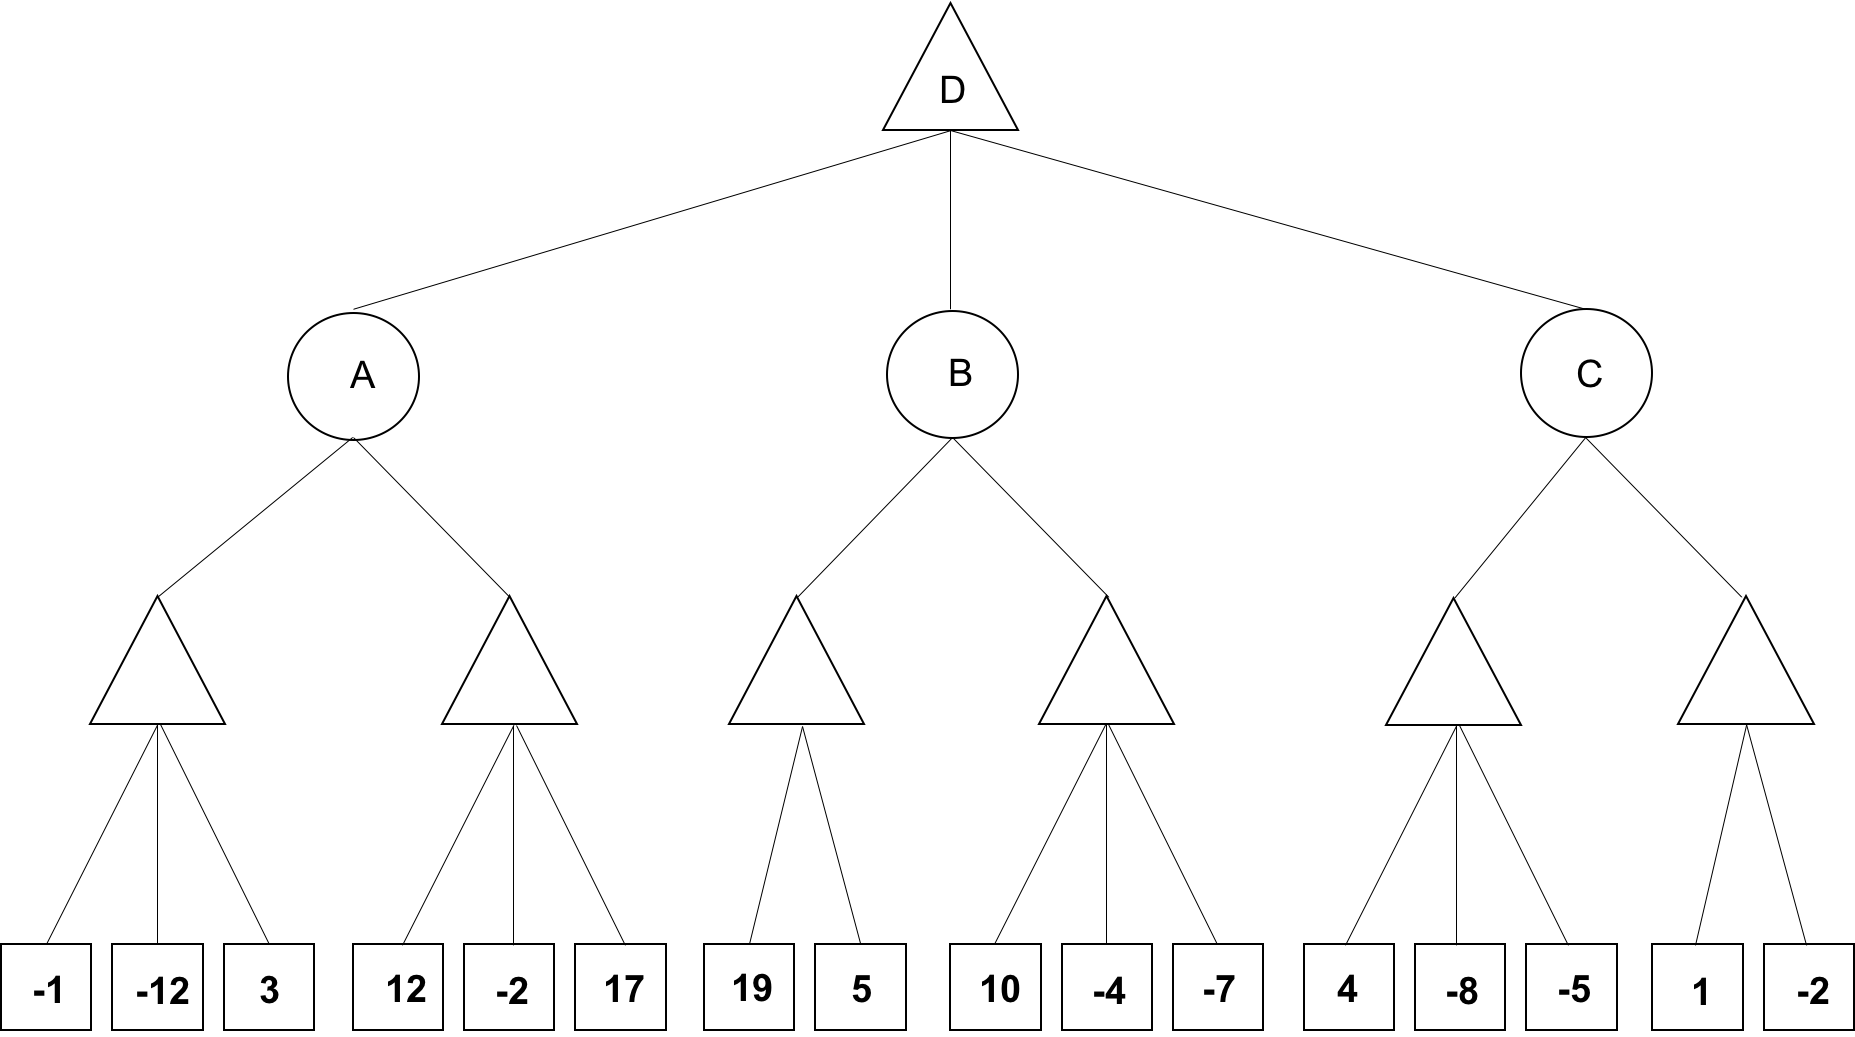
\includegraphics[width=400 pt]{figures/Expectimax-q5.png}
\end{center}

\begin{question}[2]
What is the value of node A?

\solutionspace{1.2cm}{1.5cm}{Answer:}{ \FiveA}
\end{question}

\begin{question}[2]
What is the value of node B?

\solutionspace{1.2cm}{1.5cm}{Answer:}{ \FiveB}
\end{question}

\begin{question}[2]
What is the value of node C?

\solutionspace{1.2cm}{1.5cm}{Answer:}{ \FiveC}
\end{question}

\begin{question}[2]
What is the value of node D?

\solutionspace{1.2cm}{1.5cm}{Answer:}{ \FiveD}
\end{question}

\end{problem}